\section{Manual Part Programming}
Bilet size: 61mm $\times$ 37mm $\times$ 30mm
\paragraph{3D Model}
\begin{center}
	\begin{figure}[!h]
	\centering
	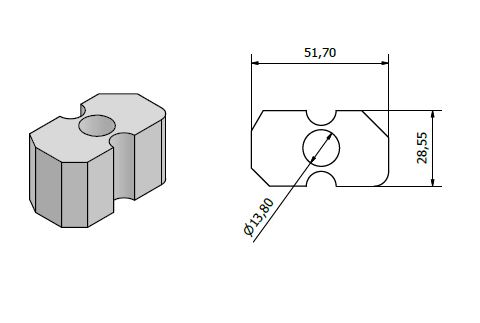
\includegraphics{Figures/3D}
	\caption[3D model]{3D Model of expected part}
	\end{figure}
\end{center}
\subsection{Process Plan}
\begin{enumerate}
\item Set bottom left corner of the part as machine zero point.
\item Clamp the workpiece on a vice on the CNC table
\item Locate the coordinates of the contours (tool path) and hole.
\item Drill the hole with a drill bit. Select a suitable spindle speed and feedrate from machinability handbook.
\item Mill using and end mill. Select a suitable spindle speed and feedrate from machinability handbook.
\end{enumerate}
\subsubsection{Coordinates of Tool Path}
\begin{center}
	\begin{figure}[!h]
	\centering
	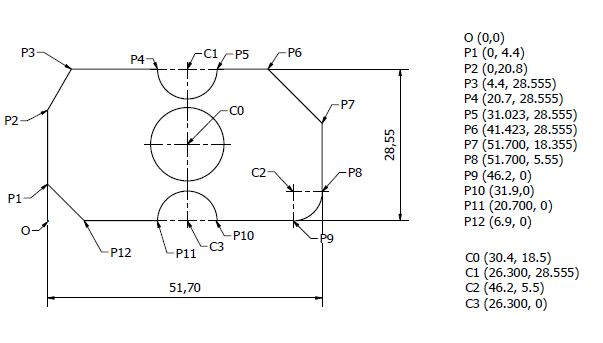
\includegraphics{Figures/Coordinates}
	\caption[Tool Path Coordinates]{Tool Path Coordinates}
	\end{figure}
\end{center}
\newpage
\subsubsection{G- and M- Codes}
\begin{table}[!h]
	\caption[G-Codes]{G-codes}
\end{table}
\begin{center}
\centering
\begin{tabular}{|l|l|}
\hline
G-code & Definition\\
\hline

G00 & Rapid Transverse\\
G01 & Linear Interpolation\\
G02 & Circular Interpolation, CW\\
G03 & Circular Interpolation, CCW\\
G21 & Input in mm\\
G28 & Return to reference point\\
G40 & Cutter diameter compensation cancel\\
G42 & Cutter compensation, right\\
G49 & Tool length compensation cancel\\
G80 & Canned Cycle cancel\\
G81 & Basic Drilling Cycle\\
G90 & Absolute Programming Mode\\
\hline
\end{tabular}
\end{center}
\begin{table}[!h]
	\caption[M-Codes]{M-codes}
\end{table}
\begin{center}
\centering
\begin{tabular}{|l|l|}
\hline
G-code & Definition\\
\hline

M00 & Program Stop\\
M02 & End of Program\\
M03 & Spindle ON, CW\\
M05 & Spindle OFF\\
M05 & Automatic Tool Change\\
M07 & Flood Coolant ON\\
M09 & Coolant OFF\\
M30 & Program Reset and Rewind\\
\hline
\end{tabular}
\end{center}
\begin{table}[!h]
	\caption[Part Program]{Part Program}
\end{table}
\centering
\begin{landscape}
\begin{longtable}{|l|l|l|l|l|l|l|l|l|l|l|l|l|l|l|l|l|}
\hline
\textbf{Description} & \textbf{N} & \textbf{G} & \textbf{G} & \textbf{G} & \textbf{X} & \textbf{Y} & \textbf{Z} & \textbf{R} & \textbf{I} & \textbf{J} & \textbf{K} & \textbf{M} & \textbf{T} & \textbf{D} & \textbf{S} & \textbf{F}\\
\hline
Program Number & 0400 &  &  &  &  &  &  &  &  &  &  &  &  &  &  & \\
\hline
Input in mm & 0100 & 21 &  &  &  &  &  &  &  &  &  &  &  &  &  & \\
\hline
Billet Size & 0110 &  &  &  & 61 & 37 & 30 &  &  &  &  &  &  &  &  & \\
\hline
Tool Definition & 0120 &  &  &  &  &  &  &  &  &  &  &  & 01 & 13.8 &  & \\
\hline
 &  &  &  &  &  &  &  &  &  &  &  &  & 01 & 13.8 &  & \\
 \hline
Cancel Cycles & 0130 & 40 & 49 & 80 &  &  &  &  &  &  &  &  &  &  &  & \\
\hline
Return to reference point & 0140 & 28 & 90 &  & 0 & 0 & 0 &  &  &  &  &  &  &  &  & \\
\hline
Tool Load & 0150 &  & & & &  & & & & & & 06 & 01 & & 1000 & 120\\
\hline
Tool Clearance height at O & 0150 & 01 & & & & & 10 & & & & & & & & &\\
\hline
Spindle ON, CW & 0160 & & & & & & & & & & & 03 & & & &\\
\hline
Flood Coolant ON & & & & & & & & & & & & 07 & & & &\\
\hline
Drill hole at C0 & 0170 & 81 & & & 30.4 & 18.5 & & 5 & & & & & & &  &\\
\hline
Return to reference point & 0180 & 01 & 28 & & 0 & 0 & Z 0 & & & & & & & & &\\
\hline
Spindle STOP & 0185 & & & & & & & & & & & 05 & & & & \\
\hline
Tool Change & 0190 &  & & & & & & & & & & 06 & 02 & & & \\
\hline
Spindle ON, CW & 0195 & & & & & & & & & & & 03 & & & &\\
\hline
\hline
\end{longtable}
\end{landscape}

\begin{landscape}
\begin{longtable}{|l|l|l|l|l|l|l|l|l|l|l|l|l|l|l|l|l|}
\hline
\textbf{Description} &\textbf{N}& \textbf{G} & \textbf{G} & \textbf{G} & \textbf{X} & \textbf{Y} & \textbf{Z} & \textbf{R} & \textbf{I} & \textbf{J} & \textbf{K} & \textbf{M} & \textbf{T} & \textbf{D} & \textbf{S} & \textbf{F}\\
\hline
Down Feed at O & 0200 & 01 & & & & & -35 & & & & & & & & &\\
\hline
Linear Interpolation to P1 & 0210 & 01 & & & 0 & 4.4 & 0 & & & & & & & & &\\
Linear Interpolation to P2 & 0220 & 01 & & & 0 & 20.8 & 0 & & & & & & & & &\\
\hline
Linear Interpolation to P3 & 0230 & 01 & & & 0 & 4.4 & 28.6 & & & & & & & & &\\
\hline
Linear Interpolation to P4 & 0240 & 01 & & & 0 & 20.7 & 28.6 & & & & & & & & &\\
\hline
Circular Interpolation to P5, CCW & 0250 & 03 & & & 31.0 & 28.6 & & & 26.3 & 28.6 & & & & & &\\
\hline
Linear Interpolation to P6 & 0260 & 01 & & & 0 & 41.4 & 28.6 & & & & & & & & &\\
\hline
Linear Interpolation to P7 & 0270 & 01 & & & 0 & 51.7 & 18.3 & & & & & & & & &\\
\hline
Linear Interpolation to P8 & 0280 & 01 & & & 0 & 51.7 & 18.4 & & & & & & & & &\\
\hline
Circular Interpolation to P9, CW & 0290 & 02 & & & 46.2 & 0 & & & 46.2 & 5.5 & & & & & &\\
\hline
Linear Interpolation to P10 & 0300 & 01 & & & 0 & 31.9 & 0 & & & & & & & & &\\
\hline
Circular Interpolation to P11, CCW & 0310 & 03 & & & 20.7 & 0 & & & 26.3 & 0 & & & & & &\\
\hline
Linear Interpolation to P12 & 0300 & 01 & & & 0 & 6.9 & 0 & & & & & & & & &\\
\hline
Return to reference point & 0310 & 01 & 28 & & 0 & 0 &  0 & & & & & & & & &\\
\hline
Spindle STOP & 0320 & & & & & & & & & & & 05 & & & & \\
\hline
Coolant OFF & & & & & & & & & & & & 09 & & & &\\
\hline
Program Reset and Rewind & 0320 & & & & & & & & & & & 30 & & & & \\
\hline
\hline
\end{longtable}
\end{landscape}